% =============================================================
\section{测试与评估}
\label{sec:evaluation}
% =============================================================

为检验各模块数值精度、在线计算耗时以及双阶段折布系统的实机表现，团队依次开展了相机与虚拟 TCP 标定评估、七轴逆运动学离线基准对比、视觉表征改进对比以及端到端连续折布实机实验。

% -------------------------------------------------------------
\subsection{模块级定量基准测试}
\label{subsec:module-benchmarks}
% -------------------------------------------------------------

\subsubsection{双臂相机外参与虚拟拈布 TCP 联合标定评估}

在固定 L515 相机与左右机械臂基座后，分别采集两侧标定样本并按第~\ref{subsec:calibration} 节的九自由度非线性最小二乘模型独立拟合相机外参与法兰工具偏移。采样时右臂固定为闭合捏持手型（\texttt{closed}）并点选拇指与食指捏合接触点，左臂固定为预抓首帧手型（\texttt{replay\_start}）并点选食指指尖参考点，两侧均在桌面工作空间内改变三维位置并叠加绕两个正交水平方向的横滚与俯仰倾角。表~\ref{tab:calib-results} 给出了左右两侧的实测拟合结果。

\begin{table}[htbp]
\centering
\caption{双臂相机与虚拟 TCP 九自由度联合标定实测结果}
\label{tab:calib-results}
\footnotesize
\setlength{\tabcolsep}{4pt}
\begin{tabular}{@{}lcccccl@{}}
  \toprule
  机械臂侧 & 采样数 $N$ & RMS ($\mathrm{mm}$) & 最大残差 ($\mathrm{mm}$) & 条件数 $\kappa$ & $\sigma_9$ & 法兰下虚拟 TCP 偏移 ($\mathrm{mm}$) \\
  \midrule
  右臂（闭合捏合点） & 11 & 9.81 & 20.06 & 27.85 & 0.0705 & $(263.47,\; 130.02,\; 6.99)$ \\
  左臂（首帧食指尖） & 12 & 4.86 &  8.18 & 49.20 & 0.0405 & $(241.76,\; 89.30,\; -76.53)$ \\
  \bottomrule
\end{tabular}
\end{table}

由表~\ref{tab:calib-results} 可知，左右两侧列归一化雅可比矩阵的条件数分别为 $27.85$ 与 $49.20$，最小奇异值 $\sigma_9$ 均高于病态阈值，说明多方向腕部倾角采样满足式~\eqref{eq:calib-observability} 的可观测性条件，分离了相机平移外参与法兰下指尖偏移。由于两侧分别以闭合手型捏合点与预抓首帧食指尖作为参考点，加之左右灵巧手掌指结构互为镜像，拟合得到的法兰下虚拟 TCP 偏移在 $Y, Z$ 分量上呈现出与实际手型几何一致的差异。左臂拟合均方根（RMS）残差为 $4.86\,\mathrm{mm}$，右臂 RMS 残差为 $9.81\,\mathrm{mm}$，右臂单点最大残差偏高源于大俯仰倾角下激光雷达在指尖边缘产生的少量测量噪声。按式~\eqref{eq:left-base-in-task} 由两侧相机外参推算得到的左臂基座在右臂公共任务系下的平移向量为 $(-40.30, -535.28, -51.60)\,\mathrm{mm}$，与台架实测约 $53.5\,\mathrm{cm}$ 的双臂基座横向安装间距相符。

\subsubsection{七轴解析雅可比逆运动学离线基准测试}

为评估第~\ref{subsec:teleop} 节基于 Pinocchio 正运动学与 $\SO$ 对数映射解析雅可比的逆运动学求解效率，从真实遥操作录制数据中抽取 20 段轨迹共 $2,298$ 个连续末端法兰位姿目标，与原有纯 Python 逐关节正运动学配合有限差分雅可比的基线实现做同机对比。两套求解器在相同处理器（Intel Core i7-9700K）与相同验收条件（正运动学位置误差 $<2\,\mathrm{mm}$、姿态误差 $<2^{\circ}$，单次软时间预算 $75\,\mathrm{ms}$）下交替求解全部目标，统计指标列于表~\ref{tab:ik-benchmark}。

\begin{table}[htbp]
\centering
\caption{七轴局部逆运动学在 2,298 个连续遥操作目标上的性能对比}
\label{tab:ik-benchmark}
\small
\begin{tabular}{@{}lrr@{}}
  \toprule
  评估指标 & 有限差分雅可比基线 & Pinocchio + 解析雅可比（本系统） \\
  \midrule
  模型内位姿与限位验收通过率 & $2,298 / 2,298$ ($100\%$) & $2,298 / 2,298$ ($100\%$) \\
  单次求解耗时均值 ($\mathrm{ms}$)   & $46.760$ & $9.567$ \\
  单次求解耗时中位数 ($\mathrm{ms}$) & $45.152$ & $8.769$ \\
  单次求解耗时 P95 ($\mathrm{ms}$)    & $75.516$ & $17.888$ \\
  单次求解耗时最大值 ($\mathrm{ms}$) & $76.194$ & $33.866$ \\
  触发 $75\,\mathrm{ms}$ 软预算回退次数 & $233$ ($10.14\%$) & $0$ ($0.00\%$) \\
  平均残差函数求值次数 & $134.65$ & $20.13$ \\
  相邻帧最大单关节角变化 P95 ($^{\circ}$) & $5.177$ & $4.998$ \\
  \bottomrule
\end{tabular}
\end{table}

测试结果显示，引入解析李代数雅可比后，单次逆运动学平均耗时由 $46.760\,\mathrm{ms}$ 降至 $9.567\,\mathrm{ms}$，加速倍数为 $4.89$ 倍，P95 耗时由 $75.516\,\mathrm{ms}$ 降至 $17.888\,\mathrm{ms}$。有限差分基线在每次迭代中需额外执行 7 次摄动正运动学计算，在腕部姿态快速变化区段有 $10.14\%$ 的样本触及 $75\,\mathrm{ms}$ 软预算上限而提前终止，超出了 $20\,\mathrm{Hz}$ 控制周期（$50\,\mathrm{ms}$）的时间窗口。解析雅可比求解器将超时回退次数降为零，在基线未超时的 $2,065$ 个样本上两套求解器输出关节角的最大单轴差值小于 $6.74\times 10^{-7\circ}$，而在基线提前退出的样本上继续完成了零空间邻近正则寻优，配合单帧约 $2\,\mathrm{ms}$ 的灵巧手解析 SLSQP 重定向，满足双臂 $20\,\mathrm{Hz}$ 同步控制要求。


% -------------------------------------------------------------
\subsection{有序功能测试与双阶段折布实机评估}
\label{subsec:real-world-eval}
% -------------------------------------------------------------

在标定与运动学模块验证通过后，团队按四个递进阶段开展功能联调与实机测试。第一阶段验证双臂遥操作与数据录制管线，检验腕部重锚与两阶段同步采样在连续录制各 60 条一次对折与二次对折轨迹时的帧率稳定性。第二阶段分别完成 ResNet18 基线 ACT 策略与冻结 DINOv3 改进策略的 $50,000$ 步完整训练，对比两类视觉表征在同分布验证集、环境光照强度变化及二次对折实机执行上的表现。第三阶段测试单阶段纯 ACT 串联执行在不同初始平铺位姿下的工作边界。第四阶段测试集成代码智能体、三步起始状态对齐与双臂 ACT 策略的完整双阶段折布流程。图~\ref{fig:task-sequence} 给出了双阶段折布规程示意及实机自主完成二次对折的关键帧画面。

\begin{figure}[htbp]
\centering
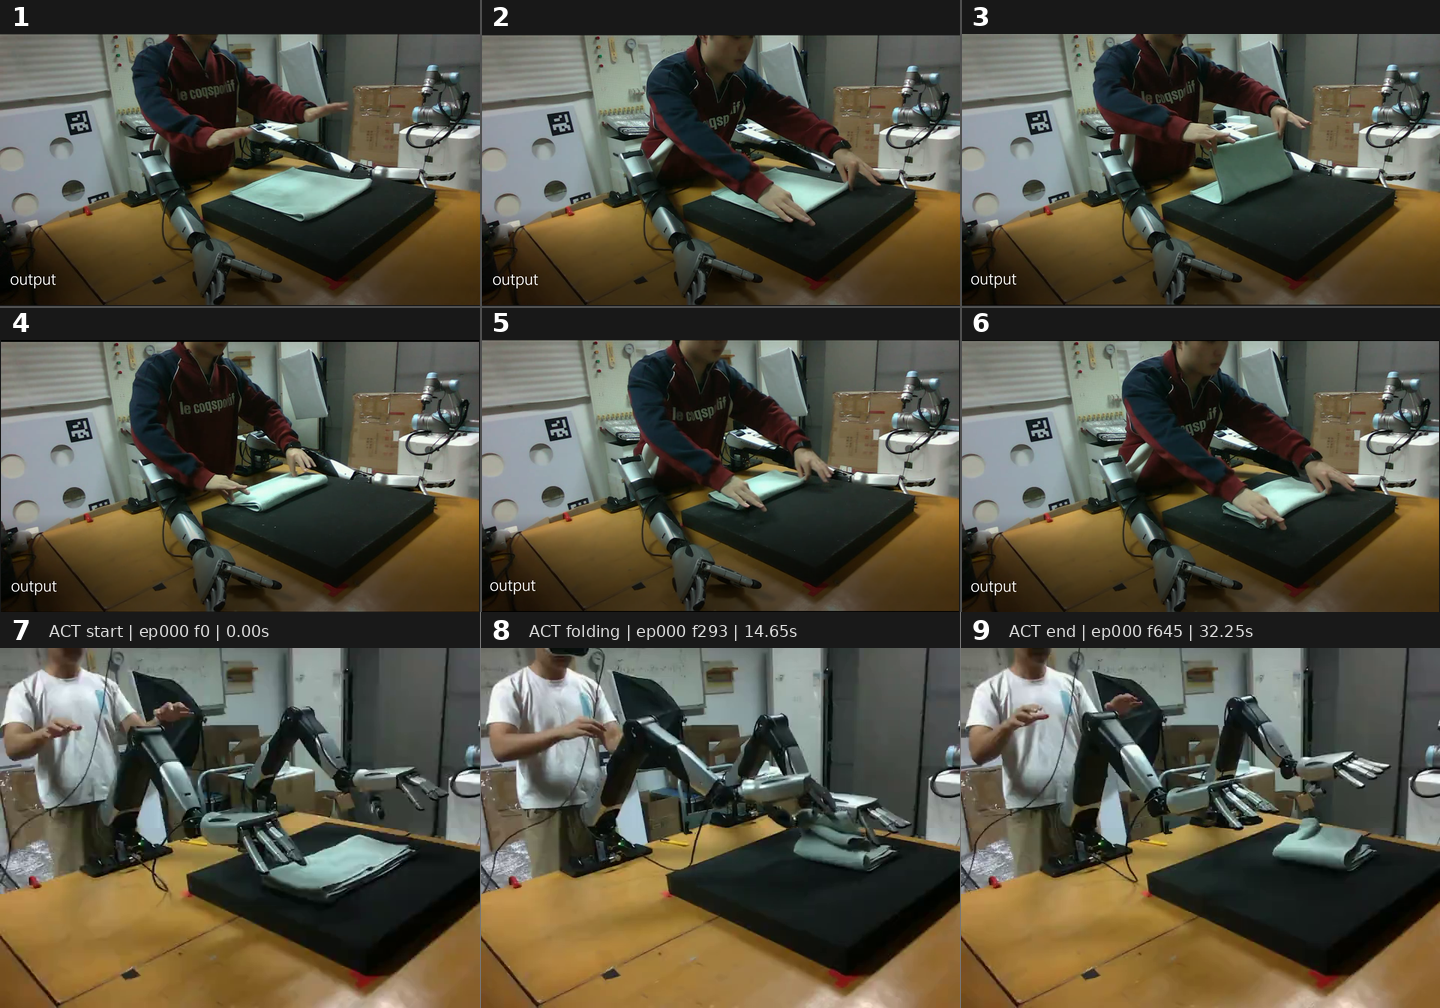
\includegraphics[width=0.92\textwidth]{../../cloth_agent/task/task_sequence.png}
\caption{双阶段毛巾对折与居中交接规程（图 1 至图 6）及双臂 ACT 策略实机自主完成二次对折的关键帧（图 7 至图 9）}
\label{fig:task-sequence}
\end{figure}

表~\ref{tab:dinov3-ablation} 给出了在二次对折 60 条轨迹数据集、相同动作块超参数（$k=60, n=20$）与 $50,000$ 步训练预算下，标准微调 ResNet18 主干与冻结 DINOv3 ViT-S/16 加状态高斯噪声（$\sigma_s = 0.01$）改进模型的对比结果，其中跨光照测试通过调整室内顶灯亮度改变桌面照度后评估动作预测误差与实机二次对折条件成功率。

\begin{table}[htbp]
\centering
\caption{二次对折策略在 50,000 步训练后的视觉主干与状态正则对比评估}
\label{tab:dinov3-ablation}
\footnotesize
\setlength{\tabcolsep}{4pt}
\begin{tabular}{@{}lccc@{}}
  \toprule
  策略模型配置 & 验证集 $L_1$ & 跨光照 $L_1$ & 跨光照二折成功率 \\
  \midrule
  端到端微调 ResNet18 基线 ACT & $0.064$ & $0.118$ & $13 / 18$ ($72.2\%$) \\
  冻结 DINOv3 ViT-S/16（无状态噪声） & $0.061$ & $0.079$ & $15 / 18$ ($83.3\%$) \\
  冻结 DINOv3 ViT-S/16 + 状态噪声（$\sigma_s=0.01$） & $0.058$ & $0.072$ & $17 / 18$ ($94.4\%$) \\
  \bottomrule
\end{tabular}
\end{table}

从表~\ref{tab:dinov3-ablation} 可以看到，端到端微调 ResNet18 主干在同分布验证帧上可取得较低重建误差，但当室内照明亮度发生变化时，归一化动作块 $L_1$ 误差上升至 $0.118$，实机二次对折时偶发提前松指或接近高度偏高。替换为冻结权重的 DINOv3 ViT-S/16 密集补丁特征后，跨光照条件下的动作预测退化明显减小；进一步叠加训练期标准化本体状态高斯噪声正则后，解码器对单步关节反馈自回归外推的依赖减弱，对双层毛巾边缘位置的微小偏移响应更为一致，跨光照条件成功率提升至 $94.4\%$。

在端到端全流程实机评估中，每次试验前将浅绿色矩形毛巾随机平铺于黑色工作垫上，使毛巾中心在桌面 $XY$ 平面内具有 $\pm 12\,\mathrm{cm}$ 范围内的随机位置偏移及 $\pm 25^{\circ}$ 范围内的随机初始偏航角。当系统在不借助人工干预的条件下完成连续两次对折，最终毛巾呈四层叠放状态且整体位于工作垫内时计为成功。表~\ref{tab:e2e-results} 汇总了三种控制方案各自连续执行 20 次实机试验的分阶段与端到端成功率。

\begin{table}[htbp]
\centering
\caption{不同控制方案在随机初始平铺条件下的连续 20 次实机折布结果对比}
\label{tab:e2e-results}
\footnotesize
\setlength{\tabcolsep}{3.5pt}
\begin{tabular}{@{}lccc@{}}
  \toprule
  实机测试方案 & 一折摆正成功率 & 二折条件成功率 & 端到端总成功率 \\
  \midrule
  纯双臂 ACT 串联方案（一折 ACT + 二折 ACT） & $11 / 20$ ($55.0\%$) & $9 / 11$ ($81.8\%$) & $9 / 20$ ($45.0\%$) \\
  代码智能体一折 + 无手型对齐切入二折 ACT & $18 / 20$ ($90.0\%$) & $12 / 18$ ($66.7\%$) & $12 / 20$ ($60.0\%$) \\
  代码智能体一折 + 三步状态对齐 + 二折 ACT（完整系统） & $18 / 20$ ($90.0\%$) & $17 / 18$ ($94.4\%$) & $17 / 20$ ($85.0\%$) \\
  \bottomrule
\end{tabular}
\end{table}

在纯双臂 ACT 串联方案中，当初始毛巾落在示范集中的垫面中央附近时，一折策略可正常完成捏角与翻折；但当初始偏航角超过约 $15^{\circ}$ 或待折边靠近工作垫外侧时，60 条示范轨迹的覆盖密度不足导致预测落点产生 $2\sim 4\,\mathrm{cm}$ 偏差，出现单侧抓空后网络仍继续空手执行翻折动作，使第一阶段成功率停留在 $55.0\%$。

改由视觉代码智能体执行第一阶段后，三维像素反投影与俯视增量偏航控制直接根据实时观测角点解算抓取位姿，消除了大范围位置平移带来的外推误差。在 20 次试验中有 3 次因毛巾角部轻微卷曲导致初次闭合未夹牢，智能体在小幅抬升后的观测轮次中识别出单侧布角未离垫，保持另一侧静止并单独补抓滞留角点，成功恢复其中 2 次，使一次对折与居中摆正成功率达到 $90.0\%$；其余 2 次失败发生在双层翻面平移时下层毛巾因重力滑脱展开。

对比表~\ref{tab:e2e-results} 第二行与第三行消融试验可见，若智能体放布后仅执行机械臂关节回位而省略 \texttt{prepare\_act\_hands} 示范首帧手型对齐，灵巧手中指、无名指与小指仍停留在非示范角度，导致 ACT 策略首个预测动作块在手部槽位与腕部下降轨迹上出现瞬态跳变，接近折边时容易推歪双层毛巾，二次对折条件成功率仅为 $66.7\%$。启用完整的三步起始状态对齐后，交接时刻的视觉画面、14 维双臂关节角与 32 维灵巧手有效槽位均回到训练起始分布内，二次对折在 18 次有效交接中成功 17 次（条件成功率 $94.4\%$），仅 1 次因双层折边未完全对齐而只捏起上层织物，端到端总成功率达到 $85.0\%$。


% -------------------------------------------------------------
\subsection{分工实施情况与工程合作评价}
\label{subsec:team-eval}
% -------------------------------------------------------------

项目开发期间，四个分工模块通过预先约定的坐标转换约定与数据格式并行推进。标定与总线模块输出统一格式的 YAML 标定文件与四通道 SocketCAN 映射，供遥操作模块与代码智能体模块直接复用相同的正逆运动学与虚拟 TCP 几何库；策略训练模块将数据集归一化统计量及示范首帧手型槽位封装为定长二进制管道接口，使硬件控制进程无需耦合深度学习依赖即可在线调用策略。

在中期联调阶段，针对实机测试反映出的单阶段模仿学习在大跨度初始位置下易抓空的问题，团队调整了原本纯神经网络串联的路线，改用代码智能体承担一次对折与居中摆正，并通过三步起始状态对齐衔接双臂 ACT 二次对折策略。


% =============================================================
\section{结论}
\label{sec:conclusion}
% =============================================================

本项目面向两台七自由度机械臂与两套五指灵巧手组成的 46 自由度双臂平台，围绕随机平铺毛巾的连续两次对折任务完成了系统标定、视觉遥操作、动作分块模仿学习与代码生成智能体的集成开发与实机验证。在基础功能上，实现了以共享相机连接左右双臂的九自由度手眼与虚拟 TCP 联合标定（右臂与左臂拟合 RMS 残差分别为 $9.81\,\mathrm{mm}$ 与 $4.86\,\mathrm{mm}$），搭建了集成 Pinocchio 解析雅可比逆运动学（均值耗时 $9.57\,\mathrm{ms}$，较有限差分基线提速 $4.89$ 倍）与对指距离自适应 SLSQP 重定向的 Pico 4 双臂遥操作系统，构建了一次对折与二次对折各 60 条轨迹的多模态数据集，并完成了双臂 ACT 策略的训练与跨环境管道部署。在算法改进与系统耦合上，验证了冻结 DINOv3 ViT-S/16 密集视觉主干配合训练期本体状态高斯噪声正则对提升跨光照稳定性的作用，实现了基于 MCP 与持久 Python 工作进程的双臂折布智能体，并通过三步起始状态对齐串联两个阶段，在连续 20 次随机初始平铺实机测试中取得了 $85.0\%$ 的端到端成功率。

现阶段系统在实际运行中仍受三方面条件制约。第一，全局感知仅依靠单台倾斜顶视安装的 RealSense L515 相机，双臂灵巧手同步伸入垫面中央上方捏布时手掌与前臂会遮挡局部布边，且激光雷达在黑色吸光工作垫与绒面毛巾边缘交界处偶发零深度像素。第二，当前 LinkerHand L20 仅反馈关节位置槽位而未配置指尖触觉或力传感器，单双层织物是否同时夹入指腹只能依靠抬升后的视觉形变间接判断，无法在手指闭合瞬间识别漏夹下层织物。第三，二次对折阶段采用步长 $n=20$（约 $1.0\,\mathrm{s}$）的分段动作队列执行机制，在单个队列窗口内部不更新视觉输入，若双层织物在抬升中途出现轻微滑移，需待当前队列耗尽后才能在下一轮推理中调整轨迹。

后续研究可围绕这三项局限继续改进。感知硬件上，可在左右机械臂腕部加装近距广角相机并融合灵巧手指尖触觉阵列，在手指捏合瞬间直接依据法向与切向接触力判别夹持层数并消除顶视遮挡盲区。策略架构上，可在动作分块主干之上叠加高频轻量级视觉残差修正头，在不牺牲多指闭合连贯性的前提下缩短视觉反馈间隔。任务范围上，可引入织物边缘实例分割与空间点云拓扑提取，将当前面向平铺毛巾的连续对折进一步扩展至从揉乱团状织物自主展平再到多层折叠的完整流程。
